\documentclass{beamer}

\mode<presentation>
\usepackage{amsmath,amssymb,mathtools}
\usepackage{textcomp}
\usepackage{gensymb}
\usepackage{adjustbox}
\usepackage{subcaption}
\usepackage{enumitem}
\usepackage[utf8]{inputenc}
\usepackage{amssymb}
\usepackage{newunicodechar}
\usepackage{enumitem}
\setlist{nosep} % optional: removes vertical gaps
\setlist[enumerate]{label=\arabic*)} % custom numbering if you want

\newunicodechar{√}{$\sqrt{\;}$}
\newunicodechar{✅}{\checkmark}
\newunicodechar{❌}{\texttimes}
\usepackage{multicol}
\usepackage{listings}
\usepackage{url}
\usepackage{graphicx} % <-- needed for images
\def\UrlBreaks{\do\/\do-}

\usetheme{Boadilla}
\usecolortheme{lily}
\setbeamertemplate{footline}{
  \leavevmode%
  \hbox{%
  \begin{beamercolorbox}[wd=\paperwidth,ht=2ex,dp=1ex,right]{author in head/foot}%
    \insertframenumber{} / \inserttotalframenumber\hspace*{2ex}
  \end{beamercolorbox}}%
  \vskip0pt%
}
\setbeamertemplate{navigation symbols}{}

\lstset{
  frame=single,
  breaklines=true,
  columns=fullflexible,
  basicstyle=\ttfamily\tiny   % tiny font so code fits
}

\numberwithin{equation}{section}

% ---- your macros ----
\providecommand{\nCr}[2]{\,^{#1}{#2}}
\providecommand{\nPr}[2]{\,^{#1}P_{#2}}
\providecommand{\mbf}{\mathbf}
\providecommand{\pr}[1]{\ensuremath{\Pr\left(#1\right)}}
\providecommand{\qfunc}[1]{\ensuremath{Q\left(#1\right)}}
\providecommand{\sbrak}[1]{\ensuremath{{}\left[#1\right]}}
\providecommand{\lsbrak}[1]{\ensuremath{{}\left[#1\right.}}
\providecommand{\rsbrak}[1]{\ensuremath{\left.#1\right]}}
\providecommand{\brak}[1]{\ensuremath{\left(#1\right)}}
\providecommand{\lbrak}[1]{\ensuremath{\left(#1\right.}}
\providecommand{\rbrak}[1]{\ensuremath{\left.#1\right)}}
\providecommand{\cbrak}[1]{\ensuremath{\left\{#1\right\}}}
\providecommand{\lcbrak}[1]{\ensuremath{\left\{#1\right.}}
\providecommand{\rcbrak}[1]{\ensuremath{\left.#1\right\}}}
\theoremstyle{remark}
\newtheorem{rem}{Remark}
\newcommand{\sgn}{\mathop{\mathrm{sgn}}}
\providecommand{\abs}[1]{\left\vert#1\right\vert}
\providecommand{\res}[1]{\Res\displaylimits_{#1}}
\providecommand{\norm}[1]{\lVert#1\rVert}
\providecommand{\mtx}[1]{\mathbf{#1}}
\providecommand{\mean}[1]{E\left[ #1 \right]}
\providecommand{\fourier}{\overset{\mathcal{F}}{ \rightleftharpoons}}
\providecommand{\system}{\overset{\mathcal{H}}{ \longleftrightarrow}}
\providecommand{\dec}[2]{\ensuremath{\overset{#1}{\underset{#2}{\gtrless}}}}
\newcommand{\myvec}[1]{\ensuremath{\begin{pmatrix}#1\end{pmatrix}}}
\let\vec\mathbf
% ---------------------

\title{Matgeo Presentation - Problem 8.4.24}
\author{ee25btech11021 - Dhanush sagar}

\begin{document}
	

		




%---------------- Title Page ----------------
\begin{frame}
  \titlepage
\end{frame}

%---------------- Problem Statement ----------------
\begin{frame}{Problem Statement}
If the line $x - 1 = 0$ is the directrix of the parabola 
\[
y^2 - kx + 8 = 0,
\] 
then one of the values of $k$ is:
\begin{multicols}{4}
    \begin{enumerate}
    \item 18
    \item 8
    \item 4
    \item 14
\end{enumerate}
\end{multicols}
\end{frame}

%---------------- Mathematical Formula ----------------
\begin{frame}{solution}

We are given the parabola 
\begin{align}
y^2 - kx + 8 = 0
\end{align}
with directrix \(x - 1 = 0\). Represent the parabola in matrix form:
\begin{align}
\vec{x}^\top V \vec{x} + 2 \vec{u}^\top \vec{x} + f = 0
\end{align}



For a conic with directrix \(\vec{n}^\top \vec{x} = c\), eccentricity \(e\) and focus \(\vec{F}\), the matrix formulas are:
\begin{align}
\vec{V} &= \|\vec{n}\|^2 I - e^2 \vec{n} \vec{n}^\top \\
\vec{u} &= c e^2 \vec{n} - \|\vec{n}\|^2 \vec{F} \\
f &= \|\vec{n}\|^2 \|\vec{F}\|^2 - c^2 e^2
\end{align}

For the parabola \(y^2 - kx + 8 = 0\), we write the matrices as
\begin{align}
\vec{V} &= \myvec{0 & 0 \\ 0 & 1}, &
\vec{u} &= \myvec{-k/2 \\ 0}, &
f &= 8
\end{align}
\end{frame}
\begin{frame}{solution}

The directrix is \(\vec{n}^\top \vec{x} = c \implies \vec{n} = \myvec{1 \\ 0}, c = 1\), and for a parabola \(e = 1\). Then
\begin{align}
\vec{V} &= \|\vec{n}\|^2 I - e^2 \vec{n} \vec{n}^\top 
= 1 \cdot \myvec{1 & 0 \\ 0 & 1} - 1 \cdot \myvec{1\\0} \myvec{1 & 0} 
= \myvec{0 & 0 \\ 0 & 1}
\end{align}

The vector \(\vec{u}\) gives the focus:
\begin{align}
\vec{u} &= c e^2 \vec{n} - \|\vec{n}\|^2 \vec{F} \implies
\vec{F} = c \vec{n} - \vec{u} = \myvec{1 \\ 0} - \myvec{-k/2 \\ 0} = \myvec{1 + k/2 \\ 0}
\end{align}

The constant term is
\begin{align}
f &= \|\vec{n}\|^2 \|\vec{F}\|^2 - c^2 e^2 
= 1 \cdot \left( \myvec{1 + k/2 \\ 0}^\top \myvec{1 + k/2 \\ 0} \right) - 1 
= (1 + k/2)^2 - 1
\end{align}
\end{frame}
\begin{frame}{solution}
Equating with the given \(f = 8\):
\begin{align}
(1 + k/2)^2 - 1 &= 8 \implies (1 + k/2)^2 = 9
\end{align}

Solving the matrix equation:
\begin{align}
1 + k/2 &= 3 \implies k = 4 \\
1 + k/2 &= -3 \implies k = -8
\end{align}

Hence, one of the values of \(k\) is
\begin{align}
\boxed{4}
\end{align}\end{frame}
%---------------- C Source Code ----------------
\begin{frame}[fragile]{C Source Code:}
\begin{verbatim}
#include <stdio.h>
#include <math.h>

void generate_parabola_points(double k, double x_start,
double x_end, int n_points,double *X, double *Y) {
    double step = (x_end - x_start) / (n_points - 1);
    for(int i = 0; i < n_points; i++){
        double x = x_start + i*step;
        double y_sq = k*x - 8;  // y^2 = kx - 8
        if (y_sq >= 0) {
            X[i] = x; Y[i] = sqrt(y_sq);           // positive branch
            X[i + n_points] = x; Y[i + n_points] = -sqrt(y_sq); // negative branch
        } else {
            X[i] = X[i + n_points] = x;
            Y[i] = Y[i + n_points] = 0; // skip imaginary
        }
    }
\end{verbatim}
\end{frame}
    \begin{frame}[fragile]{C Source Code:}
\begin{verbatim}
}

// Solve for k using matrix method formulas
double solve_k_matrix() {
    double f_target = 8;
    double temp = f_target + 1;  // f = ||F||^2 - 1 => (1 + k/2)^2 = 9
    double k1 = 2*(sqrt(temp) - 1);
    double k2 = 2*(-sqrt(temp) - 1);
    printf("Possible values of k: %f , %f\n", k1, k2);
    return k1; // return first value
}






\end{verbatim}
\end{frame}

%---------------- Python solve.py ----------------
\begin{frame}[fragile]{Python Script:solve }
\begin{verbatim}
import numpy as np
import ctypes
lib = ctypes.CDLL('./libparabola.so')
n = np.array([[1], [0]])  # directrix vector
c = 1
e = 1
f_target = 8  # from parabola y^2 - kx + 8
temp = f_target + 1
k1 = 2*(np.sqrt(temp) - 1)
k2 = 2*(-np.sqrt(temp) - 1)

print("Possible k values:", k1, k2)

# Save k1 for plotting
with open("k_value.txt", "w") as f:
    f.write(str(k1))


\end{verbatim}
\end{frame}



\begin{frame}[fragile]{Python Script: plot }
\begin{verbatim}
import numpy as np
import matplotlib.pyplot as plt

k = 4  # choose k1
x = np.linspace(-5, 10, 1000)
y_square = k*x - 8

mask = y_square >= 0
x_real = x[mask]
y_real = np.sqrt(y_square[mask])
plt.plot(x_real, y_real, 'b', label=f"Parabola y^2 - {k}x + 8 = 0")
plt.plot(x_real, -y_real, 'b')
plt.axvline(x=1, color='r', linestyle='--', label='Directrix x=1')
F_x = 1 + k/2
F_y = 0





\end{verbatim}
\end{frame}
\begin{frame}[fragile]{Python Script: plot }
\begin{verbatim}
plt.plot(F_x, F_y, 'go', label='Focus')
plt.xlabel("x")
plt.ylabel("y")
plt.title("Parabola with Directrix and Focus")
plt.legend()
plt.grid(True)
plt.axis('equal')
plt.show()

\end{verbatim}
\end{frame}

\begin{frame}{Result Plot}
 \begin{figure}[H]
     \centering
     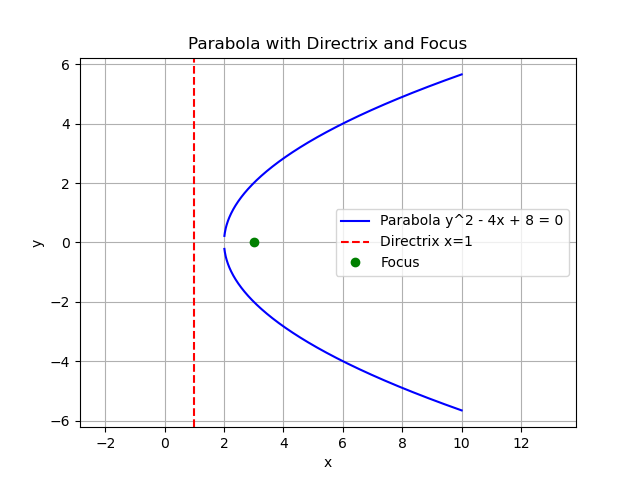
\includegraphics[width=0.8\columnwidth]{Figs/Fig1.png}
     \caption*{}
     \label{fig:fig1}
 \end{figure}
 
\end{frame}
\end{document}

